\section[Cote 81 : trois cordes autour d'un triangle]{Cote 81 : trois cordes autour d'un triangle\protect\verifie[\leanblobmain]{Folder81}}\label{sec:81}

La cote 81 n'est pas datée de sa main ; l'inventaire la date \q{à partir de 1981}, l'intitule \q{Immersions du disque et de la circonférence}, titre qu'aucun feuillet ne porte, et la range avec la cote~80 (section~\ref{sec:80}) dans le groupe \q{Géométrie et topologie combinatoire}. Les feuillets découpent : un disque le long de cordes, une sphère le long d'un graphe, des points d'un cercle en paquets. Les pages~9 et~11 sont des pages de dessins sans texte, des disques coupés de cordes avec sous chacun un petit graphe (\lot{81}{1}{9}, \lot{81}{1}{11}). La rédaction intitulée \q{Version~II} (pages~31 à~39) en cherche les axiomes.

Une \emph{décomposition binaire} d'un espace $X$ est une paire de parties fermées, les \emph{hémisphères} $\Sigma^+$ et $\Sigma^-$, de réunion $X$, non vides et distinctes (page~31). Une corde d'un disque en donne une : les deux côtés de la corde, chacun avec la corde. Deux décompositions sont \emph{non parallèles} si elles sont distinctes et si l'on peut choisir un hémisphère de chacune sans point commun (page~32, condition~(10)) : ce sont deux cordes qui ne se croisent pas. Le mot \q{non parallèle} est celui de la page ; on dit aujourd'hui \emph{compatibles}. La page~34 montre que le couple d'hémisphères disjoints est alors unique (\lot{81}{2}{34}).

Pour une famille $(\Pi_\alpha)_{\alpha \in A}$ de décompositions deux à deux non parallèles, la page~37 forme l'ensemble $C$ des hémisphères, réunion disjointe des paires $\omega_\alpha$, avec l'involution $\sigma$ qui échange les deux hémisphères d'une même décomposition, et pose (\lot{81}{2}{38})
\[
x < y \iff x \in \omega_\alpha,\ y \in \omega_\beta,\ \alpha \neq \beta \ \text{ et } \ \Sigma^x_\alpha \cap \Sigma^{\sigma y}_\beta = \emptyset. \qquad (26)
\]
Pour deux cordes qui ne se croisent pas, $x < y$ veut dire que l'hémisphère $x$ est du côté $y$ de l'autre corde. La marge ajoute \q{il faut vérifier que c'est transitif}. La page~38 abstrait alors la structure obtenue : un \emph{quartette ordonné} est un ensemble fini $C$ muni d'une involution $\sigma$ sans point fixe et d'une relation d'ordre telles que
\begin{itemize}
\item[a)] $x$ et $y$ sont comparables si et seulement si $\sigma x$ et $y$ ne le sont pas ;
\item[b)] $\sigma$ renverse l'ordre : $x < y$ entraîne $\sigma y < \sigma x$.
\end{itemize}
La condition~b) est biffée sur la page, mais son contenu revient dans le NB qui suit.

\begin{enonce}[Lecture, pages 34, 37 et 38]
Soit $(\Pi_\alpha)_{\alpha \in A}$ une famille de décompositions binaires d'un ensemble $X$, deux à deux non parallèles. Pour deux d'entre elles, le couple d'hémisphères disjoints est unique. La relation~(26) est un ordre strict sur $C = \coprod_\alpha \omega_\alpha$, $\sigma$ le renverse, et $x$, $y$ sont comparables si et seulement si $\sigma x$, $y$ ne le sont pas : $(C, \sigma, <)$ est un quartette ordonné.
\end{enonce}

\begin{proof}
Si $\Sigma_1^+ \cap \Sigma_2^+ = \emptyset$, alors $\Sigma_1^+ \subset \Sigma_2^-$ et $\Sigma_2^+ \subset \Sigma_1^-$, puisque les hémisphères de chaque décomposition recouvrent $X$. Les couples $(\Sigma_1^+, \Sigma_2^-)$ et $(\Sigma_1^-, \Sigma_2^+)$ se rencontrent donc, en $\Sigma_1^+$ et en $\Sigma_2^+$, qui sont non vides. Si $\Sigma_1^-$ et $\Sigma_2^-$ étaient aussi disjoints, on aurait de même $\Sigma_1^- \subset \Sigma_2^+$ et $\Sigma_2^- \subset \Sigma_1^+$, d'où $\Sigma_1^+ = \Sigma_2^-$ et $\Sigma_1^- = \Sigma_2^+$ : les deux décompositions seraient la même paire, ce que la non-parallélité exclut. C'est l'unicité. Pour la transitivité, $x < y$ donne $\Sigma^x \subset \Sigma^y$ par le même argument, et $y < z$ donne $\Sigma^y \cap \Sigma^{\sigma z} = \emptyset$, donc $\Sigma^x \cap \Sigma^{\sigma z} = \emptyset$. Reste à voir que $x$ et $z$ ne sont pas dans la même paire. Si $z = x$, les couples $(x, \sigma y)$ et $(\sigma x, y)$ seraient tous deux disjoints, contre l'unicité. Si $z = \sigma x$, on aurait $\Sigma^x = \Sigma^x \cap \Sigma^{\sigma z} = \emptyset$. La condition~(26) étant symétrique, $\sigma$ renverse l'ordre. Enfin, pour $x$ et $y$ dans deux paires distinctes, $x$ et $y$ sont comparables quand l'un des couples $(x, \sigma y)$, $(\sigma x, y)$ est le couple disjoint, et $\sigma x$ et $y$ le sont quand c'est l'un des couples $(\sigma x, \sigma y)$, $(x, y)$ : par l'unicité, exactement l'un des deux cas a lieu. Dans une même paire, $y$ vaut $x$ ou $\sigma x$, et $x$ n'est comparable qu'à lui-même. En Lean, ces vérifications portent sur des parties d'un ensemble quelconque.
\end{proof}

\begin{remarque}
La fermeture des hémisphères ne sert pas : la page~38 est un énoncé sur les parties d'un ensemble. La condition~b) ne se déduit pas de~a), ce qui justifie de la poser même si la page la biffe. Sur $\{x, \sigma x, y, \sigma y\}$ avec pour seules relations $x < y$ et $\sigma x < \sigma y$, la condition~a) est satisfaite et $\sigma$ ne renverse pas l'ordre. En Lean, cela se vérifie par énumération.
\end{remarque}

La page~39 énonce alors (\lot{81}{2}{39}) :
\begin{quote}
\emph{Proposition. Soit $(C, \sigma, <)$ un quartette ordonné. Alors pour tout $x \in C$, $C_{\geqslant x} = \{y \in C \mid y \geqslant x\}$ et $C_{\leqslant x} = \{y \in C \mid y \leqslant x\}$ sont totalement ordonnés.}
\end{quote}
La démonstration de la page s'arrête au milieu d'une phrase, sur \q{d'où $\sigma z <$}. Trois cordes disjointes qui entourent un triangle suffisent à réfuter l'énoncé (figure~\ref{fig:81-tripode}).

\begin{encadre}
\begin{contrexemple}[Énoncé de l'édition, page 39]
Soient trois cordes d'un disque, deux à deux disjointes, qui entourent un triangle ; notons $c_1, c_2, c_3$ les calottes qu'elles découpent et $c_1', c_2', c_3'$ les hémisphères complémentaires, qui contiennent le triangle. Les trois décompositions binaires sont deux à deux non parallèles, et leur quartette ordonné est $C = \{c_1, c_2, c_3, c_1', c_2', c_3'\}$, avec $\sigma c_i = c_i'$ et pour seules relations strictes $c_i < c_j'$ pour $i \neq j$. Alors $C_{\geqslant c_1} = \{c_1, c_2', c_3'\}$, et $c_2'$ et $c_3'$ sont incomparables.
\end{contrexemple}
\end{encadre}

\begin{proof}
Deux calottes $c_i$ et $c_j$ distinctes sont disjointes, de sorte que $c_i < \sigma c_j = c_j'$ par~(26). Les autres couples se rencontrent : $c_i'$ et $c_j'$ contiennent le triangle, et $c_i$ rencontre $c_j'$, qui la contient. Il n'y a donc pas d'autre relation, et $c_2' < c_3'$ demanderait $c_2' \cap c_3 = \emptyset$, alors que $c_3 \subset c_2'$. En Lean, la configuration est réalisée de deux façons. Comme famille de décompositions d'un modèle à sept points du disque, le triangle ouvert, les trois cordes et les trois calottes ouvertes, le calcul passe par l'énoncé précédent. Comme quartette abstrait à six éléments, les axiomes et l'incomparabilité sont décidés par énumération.
\end{proof}

\begin{figure}[htbp]
\centering
\begin{tikzpicture}[pt/.style={circle, fill, inner sep=1.3pt}, lab/.style={font=\scriptsize, inner sep=1pt}]
\begin{scope}
\draw (0,0) circle (1.6);
\foreach \a/\i in {90/1, 210/2, 330/3} {
  \draw ($(\a-55:1.6)$) -- ($(\a+55:1.6)$);
  \node[lab] at (\a:1.25) {$c_\i$};
}
\node[lab] at (0,0) {$T$};
\node[font=\small] at (0,-2.1) {trois cordes};
\end{scope}
\begin{scope}[xshift=4cm]
\node[pt] (o) at (0,0) {};
\foreach \a/\i in {90/1, 210/2, 330/3} \node[pt] (p\i) at (\a:1.1) {};
\foreach \i in {1,2,3} \draw[line width=1.6pt] (o) -- (p\i);
\node[font=\small] at (0,-2.1) {le tripode};
\end{scope}
\begin{scope}[xshift=8.2cm, x=1.1cm, y=1.5cm]
\foreach \i/\x in {1/-1, 2/0, 3/1} {
  \node (b\i) at (\x,-0.6) {$c_\i$};
  \node (t\i) at (\x,0.6) {$c_\i'$};
}
\foreach \i/\j in {1/2,1/3,2/1,2/3,3/1,3/2} \draw (b\i) -- (t\j);
\node[font=\small] at (0,-1.4) {le quartette};
\end{scope}
\end{tikzpicture}
\caption{À gauche, trois cordes disjointes autour du triangle $T$, et leurs calottes $c_1, c_2, c_3$. Au milieu, l'arbre des morceaux : un sommet par morceau, une arête par corde. C'est le tripode ; un tripode en \q{Y} épais figure parmi les graphes que Grothendieck dessine sous ses disques à la page~11 (\lot{81}{1}{11}), et la lecture l'en rapproche. À droite, le diagramme de Hasse du quartette ordonné : $c_1$ est au-dessous de $c_2'$ et de $c_3'$, qui sont incomparables. Figure de l'édition ; le croquis de la page~39 dessine les trois points $x$, $y$, $z$ de la démonstration interrompue (\lot{81}{2}{39}).}
\label{fig:81-tripode}
\end{figure}

Ce qui reste vrai est plus faible.

\begin{enonce}[Énoncé de l'édition, page 39]
Dans un quartette ordonné, tout intervalle $[x, z] = \{y \mid x \leqslant y \leqslant z\}$ est totalement ordonné. La condition~a) suffit.
\end{enonce}

\begin{proof}
Soient $x \leqslant y \leqslant z$ et $x \leqslant y' \leqslant z$, avec $y$ et $y'$ incomparables. Par~a), $\sigma y$ et $y'$ sont comparables. Si $\sigma y \leqslant y'$, alors $\sigma y \leqslant z$ : $y$ et $\sigma y$ sont tous deux comparables à $z$, ce que~a) interdit. Si $y' \leqslant \sigma y$, alors $x \leqslant \sigma y$, et $y$ et $\sigma y$ sont tous deux comparables à $x$, ce que~a) interdit aussi.
\end{proof}

\begin{remarque}
La démonstration de la page suit ce chemin : supposant $x < y$, $x < z$ et $y$, $z$ incomparables, elle obtient $\sigma y < z$, puis commence \q{d'où $\sigma z <$}. Dans le contre-exemple, avec $x = c_1$, $y = c_2'$ et $z = c_3'$, on a bien $\sigma y = c_2 < c_3' = z$ et $\sigma z = c_3 < c_2' = y$, sans contradiction : il n'y avait plus rien à trouver. Pour les familles de cordes, $C_{\geqslant x}$ est totalement ordonné pour tout $x$ quand les cordes sont en file, comme des cordes parallèles au sens usuel, et l'arbre des morceaux est alors une chaîne ; l'énoncé de la page vaut dans ce cas, qui n'est pas formalisé. Les quartettes ordonnés sont, dans le vocabulaire d'aujourd'hui, des \emph{pocsets} dont deux murs quelconques sont emboîtés, et ceux-ci sont les ensembles de demi-arbres d'un arbre fini (Dunwoody, Roller) ; l'identification n'est pas formalisée.
\end{remarque}

Les pages~40 à~52 ne gardent que les extrémités des coupures : des points rangés sur un cercle, un \emph{polygone}. Un \emph{segment} est une partie non vide et propre formée de sommets consécutifs (page~41). Soit $\Sigma$ un ensemble de segments tel que (pages~45 et~46)
\begin{itemize}
\item[($\sigma_1$)] deux éléments de $\Sigma$ qui se rencontrent sont emboîtés ;
\item[($\sigma_2$)] si $A \subsetneq B$ dans $\Sigma$, $A$ ne contient aucune extrémité de $B$ ;
\item[($\sigma_3$)] le résidu $Z = S \smallsetminus \bigcup_{A \in \Sigma} A$ n'est pas un segment.
\end{itemize}
Le \emph{cœur} de $A \in \Sigma$ est $A^* = A \smallsetminus \bigcup_{B \subsetneq A} B$. Les cœurs, avec $Z$, forment une partition non croisée du polygone. La page~47 se demande si la partition redonne la famille, et répond par un NB (\lot{81}{3}{47}) :
\begin{quote}
\emph{NB En fait, avec les seules conditions $\sigma_1$ à $\sigma_3$ sur $\Sigma$, il n'est pas vrai que la connaissance de $\widehat{\Sigma}^*$ redonne $\Sigma$, exemple la relation d'équivalence $R$ avec trois classes $\{a_1, a_1'\}$, $\{b, b'\}$, $\{a_2, a_2'\}$.}
\end{quote}

\begin{enonce}[Grothendieck, page 47]
Sur l'hexagone $a_1, b, a_2, a_2', b', a_1'$, les familles
\[
\Sigma_1 = \bigl\{\{a_1, a_1'\}, \{a_2, a_2'\}, \{a_1, a_1', b, b'\}\bigr\}, \qquad \Sigma_2 = \bigl\{\{a_1, a_1'\}, \{a_2, a_2'\}, \{a_2, a_2', b, b'\}\bigr\}
\]
sont distinctes, satisfont $(\sigma_1)$ à $(\sigma_3)$, recouvrent l'hexagone, et ont la même partition en cœurs $\{a_1, a_1'\}$, $\{b, b'\}$, $\{a_2, a_2'\}$.
\end{enonce}

\begin{proof}
Les paires $\{a_1, a_1'\}$ et $\{a_2, a_2'\}$ sont des arêtes de l'hexagone, et $\{a_1, a_1', b, b'\}$ est le segment $b', a_1', a_1, b$, d'extrémités $b$ et $b'$. Les deux petits segments sont disjoints, le premier est intérieur au grand et le second lui est disjoint : $(\sigma_1)$ et $(\sigma_2)$ sont satisfaites, et la réunion est l'hexagone, de sorte que $Z = \emptyset$, qui n'est pas un segment. Le cœur du grand segment est $\{b, b'\}$, et les deux autres sont leur propre cœur. La famille $\Sigma_2$ est l'image de $\Sigma_1$ par la symétrie qui échange $a_1$ et $a_2$. En Lean, le polygone est $\mathbb Z/6$, et les conditions et les cœurs sont calculés par énumération.
\end{proof}

\begin{figure}[htbp]
\centering
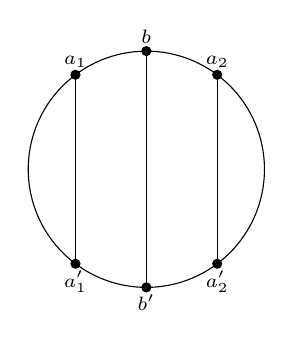
\begin{tikzpicture}[pt/.style={circle, fill, inner sep=1.3pt}, lab/.style={font=\scriptsize, inner sep=1pt}]
\draw (0,0) circle (1.5);
\foreach \x/\u/\d in {-0.9/a_1/a_1', 0/b/b', 0.9/a_2/a_2'} {
  \pgfmathsetmacro{\y}{sqrt(1.5*1.5-\x*\x)}
  \draw (\x,\y) -- (\x,-\y);
  \node[pt] at (\x,\y) {}; \node[pt] at (\x,-\y) {};
  \node[lab, anchor=south] at (\x,\y+0.05) {$\u$};
  \node[lab, anchor=north] at (\x,-\y-0.05) {$\d$};
}
\end{tikzpicture}
\caption{Les trois cordes parallèles de la page~47, $a_1a_1'$, $bb'$ et $a_2a_2'$ : la partition non croisée en trois paires vient de deux familles de segments, selon que le grand segment entoure la corde $a_1a_1'$ ou la corde $a_2a_2'$. Figure de l'édition ; Grothendieck dessine ce cercle à droite du NB (\lot{81}{3}{47}), et une rangée de disques à quatre cordes parallèles marquée d'un \q{?} à la page~9 (\lot{81}{1}{9}).}
\label{fig:81-cordes}
\end{figure}

Ne sont pas démontrés ici : la correspondance entre cartes sphériques repérées et fonctions de Belyi de la page~2, et l'action de $\mathrm{Gal}(\overline{\mathbb Q}/\mathbb Q)$ de la page~4 ; le dénombrement des morceaux et le lemme de l'arbre de la Version~I (pages~16 à~24) ; la réciproque qu'annonce l'\q{Inversement} de la page~38, que tout quartette ordonné provient d'une famille strictement non parallèle ; l'équivalence des conditions a) à c') de la page~43 ; l'existence d'au moins deux anglets d'une partition non croisée qui n'est pas grossière (page~49), et l'effeuillage des pages~49 et~50 ; le bilan des faces et du genre de l'attachement de deux arêtes (page~53).
